% a313ee25-d10e-46b1-aa73-f7151edb19a8
%
% Although we try to provide a template that completely
% matches the corresponding assignment, we do expect you
% to check that you have indeed answered all questions.
%

% ALSO VERY IMPORTANT:
% This is just a template to help you with the LaTeX part of the assignment.
% So you may change it completely according to your own wishes!
%

\documentclass[a4paper]{article}
% Typically the 'article' class is appropriate for assignments.
% And we print it on a4, so we include that as well.

\usepackage{a4wide}
% To decrease the margins and allow more text on a page.

\usepackage{graphicx}
% To deal with including pictures.

\usepackage{enumerate}
% To provide a little bit more functionality than with LaTeX's default
% enumerate environment.

\usepackage{array}
% To provide a little bit more functionality than with LaTeX's default
% array environment.

\usepackage[american]{babel}
% Use this if you want to write the document in US English. It takes care of
% (usually) proper hyphenation.
% If you want to write your answers in Dutch, please replace 'american'
% by 'dutch'.
% Note that after a change it may be that the first compilation of LaTeX
% fails. That is normal and caused by the fact that in auxiliary files
% from previous runs, there may still be a \selectlanguage{american}
% around, which is invalid if 'american' is not incorporated with babel.

\usepackage{amssymb}
% This package loads mathematical things like the fonts for the blackboard
% bold for the set of natural numbers.
\usepackage{amsmath}
% And some student asked me to include amsmath as well...

\usepackage{tikz}
\usetikzlibrary{arrows}
\usetikzlibrary{positioning}
% The tikz package can be used to draw all kinds of diagrams.
% In this assignment it is being used for drawing the parse trees.

\usepackage[all]{xy}
% Instead of tikz you can also use xy to draw parse trees with


\usepackage{xspace}
% xspace can be used to let LaTeX decide whether a command should be followed
% y a space or not, depending on what follows.

% Some obscure definition to create a circled node within xy.
% The definition is made by Freek Wiedijk who prefers to do his definitions
% in TeX instead of LaTeX, which explains the \def instead of \newcommand.
\def\node{*++[o][F-]}
\def\fnode{*++[o][F=]}

\usepackage{csquotes}

\newcommand{\exercise}[2]{\subsection*{Exercise #1}{#2}}
\newcommand{\exerciseenum}[2]{\subsection*{Exercise #1}{\begin{enumerate}[a)]#2\end{enumerate}}}
% We defined our own commands to make it easy to present all the
% exercises in the same style. The first one does not automatically
% start an 'enumerate' list, the second one does.
% The [2] means that our command needs two arguments.
% The #1 and the #2 indicate where we use these arguments in the
% command.
% There are several ways to have automatic numbering for the exercises,
% but here we have chosen to use a subsection for this and use manual
% numbering. This is because maybe not everyone will be able to do hand in
% all exercises.
% Note that we add the '*' to make sure that the subsection is not numbered.
% (Since we don't have a \section, the numbers for a subsection would be
% ugly like 0.1, 0.2 et cetera.
% The environment 'enumerate' automatically numbers the items in this list.
% The optional [a)] makes sure that the list will be like a), b), c) et cetera.



\newcommand{\abs}[1]{\ensuremath{\left|\, #1 \,\right|}}
\newcommand{\floor}[1]{\ensuremath{\left\lfloor\, #1 \,\right\rfloor}}
\newcommand{\ceil}[1]{\ensuremath{\left\lceil\, #1 \,\right\rceil}}
% Abbreviations for the absolute value, ceil and floor function.

\newcommand{\set}[1]{\ensuremath{\left\{{#1}\right\}}}
% This command puts curly braces around its argument, so it becomes
% a set. The \left and \right make sure that the braces grow in size
% if the contents of the set are large symbols.

\newcommand{\setbuild}[2]{\ensuremath{\set{{#1}\mid{#2}}}}
% We also introduce a shortcut for using the set builder notation.
% Do you understand what it does?

\newcommand{\seq}[1]{\ensuremath{\left\{{#1}\right\}}}
% This puts curly braces to define a sequence.
% Note that this is the same as the definition for a \set.

% And the next series of commands gives you some of the default sets
% that were in the slides.
\newcommand{\TT}{\ensuremath{\mathbb{T}}}
\newcommand{\FF}{\ensuremath{\mathbb{F}}}
\newcommand{\NN}{\ensuremath{\mathbb{N}}}
\newcommand{\NNp}{\ensuremath{\mathbb{N}^{+}}}
\newcommand{\ZZ}{\ensuremath{\mathbb{Z}}}
\newcommand{\ZZp}{\ensuremath{\mathbb{Z}^{+}}}
\newcommand{\QQ}{\ensuremath{\mathbb{Q}}}
\newcommand{\QQp}{\ensuremath{\mathbb{Q}^{+}}}
\newcommand{\RR}{\ensuremath{\mathbb{R}}}
\newcommand{\RRp}{\ensuremath{\mathbb{R}^{+}}}
\newcommand{\CC}{\ensuremath{\mathbb{C}}}

% And the next command gives a shorthand for the power set of a given set.
\newcommand{\power}[1]{\ensuremath{{\cal P}\left({#1}\right)}}

% The following two commands can be used to get an upright T or F, even
% when in math mode.
\newcommand{\Tt}{\ensuremath{\mathrm T}}
\newcommand{\Ff}{\ensuremath{\mathrm F}}

% We want to have a good way of presenting the | relation.
\DeclareMathOperator{\divides}{\mid}

% And we also want to have an easy way to create a bold mod as operator.
\DeclareMathOperator{\emod}{\mathbf{mod}}

% And in addition we want to have a non bold version for (mod n).
\newcommand{\tmod}{\mbox{mod}\xspace}

% We create an environment for numbered theorems.
\newtheorem{theorem}{Theorem}

% And we create a \templtag command for referring to the template.
\newcommand{\templtag}[1]{\marginpar{\fbox{#1}}}

% This command puts a `def' on top of an `='.
\newcommand{\isdef}{\ensuremath{\,\,\buildrel\rm def\over=}\,\,}

\reversemarginpar
\title{Mathematical Structures\\Assignment 7}

% Replace the placeholders by your real name, student number and
% group (for the exercise hours)
\author{Tony Lopar \\ s1013792 \quad Group 1}

% In LaTeX everything before \begin{document} is called pre-amble.
% This is where you put all important settings. The real document
% starts after \begin{document}.
\begin{document}
\maketitle
% \maketitle makes sure that the title is shown on the first page of
% the document.


% Now we use the command we defined earlier and give it the proper two
% parameters.
% Because the second parameter is long, we put a % directly after the
% opening curly brace {. This is not needed but makes the source file
% look a bit better.
\exerciseenum{12}{%
\addtocounter{enumi}{3}
\item%d
\begin{description}
\item[Reflexive]
The relation $R$ is reflexive.
Let $f$ be a function from $\ZZ$ to $\ZZ$.
Then $R(f,f)$ holds, because $f - f = 0$ and $0 \in \ZZ$.

\item[Symmetric]
The relation $R$ is symmetric.
If we have (f, g) the relation will be $f - g = C$ and (g, f) will be $g - f = C$ which will both give $C \in \ZZ$.
\item[Transitive]
The relation $R$ is transitive.
Let's assume we also have a function h for which $R(g, h)$ holds. We already know that $(f, g)$ results a $C \in \ZZ$. Knowing these two relations, we also know that $(f, h) = C \in \ZZ$ will hold.
\end{description}
\item%e
\begin{description}
\item[Reflexive]
The relation $R$ is reflexive.
Then $R(f,f)$ holds, because f is equal to itself.
\item[Symmetric]
The relation $R$ is symmetric.
The \enquote{=} implies that when $f = g$, $g = f$ also follows.
\item[Transitive]
The relation $R$ is transitive.
When we know that $(f, g)$ and have an h for which $(g, h)$, then we also know that $(f, h)$ because of the transivity of the \enquote{=}.
\end{description}
}

\exercise{13}{%
The depicted relation is an equivalence relation, because:
% Perhaps you can use the description environment as given below?
% Make sure that you don't do too much work!

\begin{description}
\item[Reflexive]
The depicted relation is reflexive, because every element points to itself which means it has a relation with itself.
\item[Symmetric]
The depicted relation is symmetric.
Because for every relation with a different node, there is also a relation to the other side.
\item[Transitive]
The depicted relation is transitive.
The graph is split into two parts, from every vertex we have a relationship with all other vertices in that part. For example, we have $(a, d)$ and $(d, a)$. We know that $(a, a)$, because we can reach all points from the other point in the relation.
\end{description}
}


\exerciseenum{14}{%
\addtocounter{enumi}{2}
\item%c
The equivalence class $[7]_{\dagger}$ is the set of all positive
integers such that the integers have the same amount of unique, positive divisors.

Therefore the elements in the set have two divisors, since 7 has only itself and 1 as positive divisor. This means the set will consist of primes. A subset with four elements of the set is as follows: $\{2, 3, 5, 11\}$.
}


\exerciseenum{15}{%
\item%a
We define the equivalence relation $\sim$ on $\NN$ by
\[
n \sim m  \isdef  n + 23m
\]
% Note that you don't have to prove that it is an equivalence relation.
% But you do have to explain something about the quotient set.
This gives the equivalent classes:
\begin{eqnarray*}
[0]_{\sim} &=&  \set{0, 23, 46, 69, \dots} \\
{[1]_{\sim}} &=&  \set{1, 24, 47, 70, \dots} \\
{[2]_{\sim}} &=&  \set{2, 25, 48, 71, \dots} \\
\vdots &=&  \vdots
\end{eqnarray*}
Hence the quotient set $\NN/\sim$ is \dots

\item%b
We define the equivalence relation $\sim$ on $\NN$ by
\[
n \sim m  \isdef  n = m
\]
This gives the equivalent classes:
\begin{eqnarray*}
[0]_{\sim} &=&  \set{0} \\
{[1]_{\sim}} &=&  \set{1} \\
{[2]_{\sim}} &=&  \set{2} \\
\vdots &=&  \vdots
\end{eqnarray*}

\addtocounter{enumi}{1}
\item%d
We define the equivalence relation $\sim$ on $\NN$ by
\[
n \sim m  \isdef  n = 0 \land m = 0
\]

This gives the equivalent classes:
\begin{eqnarray*}
[0]_{\sim} &=&  \set{0} \\
{[1]_{\sim}} &=&  \set{1, 2, 3, 4, \dots}
\end{eqnarray*}
Hence the quotient set $\NN/\sim$ is \dots
}


\exerciseenum{16}{%
\item%a
$(\RR,=)$
is a poset, because the relations meets the following requirements:
%Either (if it is a poset) give a proof that it meets all the
%requirements.
%Or (if it is not a poset) give a counterexample showing that not all
%requirements are met.
\begin{description}
\item[Reflexive]
The relation is reflexive, because every element is equal to itself and thus has a relation with itself.
\item[Anitsymmetric]
The relation is antisymmetric.
The only relations are when $a = b$. This means we cannot have a case where $R(a,b)$ and $R(b, a)$ where $a \neq b$.

\item[Transitive]
The relation is transitive.
The \enquote{=} has a transitive property. This means when we have $a = b$ and $b = c$, then $a = c$ follows.

\end{description}

\addtocounter{enumi}{1}
\item%c
$(\RR,\leq)$
is a poset, because:
\begin{description}
\item[Reflexive]
The relation is reflexive, because for every element $a \in \RR$ it holds that $a \leq a$.
\item[Anitsymmetric]
The relation is antisymmetric.
The only elements for which $a \leq b$ and $b \leq a$ holds are elements for which $a = b$. When we have that $a \neq b$, then if $a \leq b$, then $b > a$. This means it's only symmetric when $a = b$.

\item[Transitive]
The relation is transitive.
Let's assume we have three elements $a, b, c \in \RR$. If $a \leq b$ and $b \leq c$, then $a \leq c$ also holds because the $\leq$ is transitive.

\end{description}
}

\exercise{17}{%
This is the Hasse diagram we are talking about:
\begin{center}
\scalebox{0.8}{%
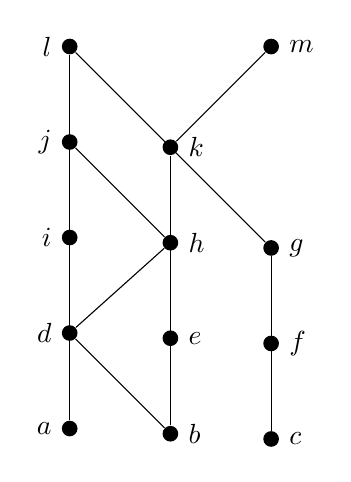
\begin{tikzpicture}[
nodot/.style={
  circle,
},
mydot/.style={
  circle,
  fill,
  inner sep=2pt
},
%>=latex,
%shorten >= 3pt,
%shorten <= 3pt
]
\node[mydot,label={left:$l$}] (l) {};
\node[mydot,below=of l,label={left:$j$}] (j) {};
\node[mydot,below=of j,label={left:$i$}] (i) {};
\node[mydot,below=of i,label={left:$d$}] (d) {};
\node[mydot,below=of d,label={left:$a$}] (a) {};

\node[nodot,right=of l] (in1) {};
\node[mydot,below=of in1,label={right:$k$}] (k) {};
\node[mydot,below=of k,label={right:$h$}] (h) {};
\node[mydot,below=of h,label={right:$e$}] (e) {};
\node[mydot,below=of e,label={right:$b$}] (b) {};

\node[mydot,right=of in1,label={right:$m$}] (m) {};
\node[nodot,below=of m] (in2) {};
\node[mydot,below=of in2,label={right:$g$}] (g) {};
\node[mydot,below=of g,label={right:$f$}] (f) {};
\node[mydot,below=of f,label={right:$c$}] (c) {};

\path (a) edge (l);
\path (b) edge (k);
\path (c) edge (g);
\path (b) edge (d);
\path (d) edge (h);
\path (h) edge (j);
\path (g) edge (l);
\path (k) edge (m);
\end{tikzpicture}
}
\end{center}
\begin{enumerate}[a)]
\addtocounter{enumi}{1}
\item%b
The minimal elements are a, b and c

\item%c
There is no greatest element, because the elements l and m are incomparable.

\addtocounter{enumi}{2}
\item%f
The least upperbound of $\{a,b,c\}$ exists and it is k,
because a, b and c can be compared to k and k is lower than the other bounds l and m.
\item%g
There are no lower bound, because h and g are incomparable for the elements below.
\end{enumerate}
}

\exerciseenum{18}{%
\addtocounter{enumi}{1}
\item%b
Suppose $\bowtie$ is an arbitrary relation on $V$ that is left-total,
symmetric and transitive.
We are going to prove that $\bowtie$ is an equivalence relation,
by showing that it is also reflexive. This is a case, since for all elements in the set V, the same element exists in this same set which was a property of left-total.
}
\end{document}
